\documentclass[twoside]{book}

% Packages required by doxygen
\usepackage{fixltx2e}
\usepackage{calc}
\usepackage{doxygen}
\usepackage[export]{adjustbox} % also loads graphicx
\usepackage{graphicx}
\usepackage[utf8]{inputenc}
\usepackage{makeidx}
\usepackage{multicol}
\usepackage{multirow}
\PassOptionsToPackage{warn}{textcomp}
\usepackage{textcomp}
\usepackage[nointegrals]{wasysym}
\usepackage[table]{xcolor}

% Font selection
\usepackage[T1]{fontenc}
\usepackage[scaled=.90]{helvet}
\usepackage{courier}
\usepackage{amssymb}
\usepackage{sectsty}
\renewcommand{\familydefault}{\sfdefault}
\allsectionsfont{%
  \fontseries{bc}\selectfont%
  \color{darkgray}%
}
\renewcommand{\DoxyLabelFont}{%
  \fontseries{bc}\selectfont%
  \color{darkgray}%
}
\newcommand{\+}{\discretionary{\mbox{\scriptsize$\hookleftarrow$}}{}{}}

% Page & text layout
\usepackage{geometry}
\geometry{%
  a4paper,%
  top=2.5cm,%
  bottom=2.5cm,%
  left=2.5cm,%
  right=2.5cm%
}
\tolerance=750
\hfuzz=15pt
\hbadness=750
\setlength{\emergencystretch}{15pt}
\setlength{\parindent}{0cm}
\setlength{\parskip}{3ex plus 2ex minus 2ex}
\makeatletter
\renewcommand{\paragraph}{%
  \@startsection{paragraph}{4}{0ex}{-1.0ex}{1.0ex}{%
    \normalfont\normalsize\bfseries\SS@parafont%
  }%
}
\renewcommand{\subparagraph}{%
  \@startsection{subparagraph}{5}{0ex}{-1.0ex}{1.0ex}{%
    \normalfont\normalsize\bfseries\SS@subparafont%
  }%
}
\makeatother

% Headers & footers
\usepackage{fancyhdr}
\pagestyle{fancyplain}
\fancyhead[LE]{\fancyplain{}{\bfseries\thepage}}
\fancyhead[CE]{\fancyplain{}{}}
\fancyhead[RE]{\fancyplain{}{\bfseries\leftmark}}
\fancyhead[LO]{\fancyplain{}{\bfseries\rightmark}}
\fancyhead[CO]{\fancyplain{}{}}
\fancyhead[RO]{\fancyplain{}{\bfseries\thepage}}
\fancyfoot[LE]{\fancyplain{}{}}
\fancyfoot[CE]{\fancyplain{}{}}
\fancyfoot[RE]{\fancyplain{}{\bfseries\scriptsize Generated by Doxygen }}
\fancyfoot[LO]{\fancyplain{}{\bfseries\scriptsize Generated by Doxygen }}
\fancyfoot[CO]{\fancyplain{}{}}
\fancyfoot[RO]{\fancyplain{}{}}
\renewcommand{\footrulewidth}{0.4pt}
\renewcommand{\chaptermark}[1]{%
  \markboth{#1}{}%
}
\renewcommand{\sectionmark}[1]{%
  \markright{\thesection\ #1}%
}

% Indices & bibliography
\usepackage{natbib}
\usepackage[titles]{tocloft}
\setcounter{tocdepth}{3}
\setcounter{secnumdepth}{5}
\makeindex

% Hyperlinks (required, but should be loaded last)
\usepackage{ifpdf}
\ifpdf
  \usepackage[pdftex,pagebackref=true]{hyperref}
\else
  \usepackage[ps2pdf,pagebackref=true]{hyperref}
\fi
\hypersetup{%
  colorlinks=true,%
  linkcolor=blue,%
  citecolor=blue,%
  unicode%
}

% Custom commands
\newcommand{\clearemptydoublepage}{%
  \newpage{\pagestyle{empty}\cleardoublepage}%
}

\usepackage{caption}
\captionsetup{labelsep=space,justification=centering,font={bf},singlelinecheck=off,skip=4pt,position=top}

%===== C O N T E N T S =====

\begin{document}

% Titlepage & ToC
\hypersetup{pageanchor=false,
             bookmarksnumbered=true,
             pdfencoding=unicode
            }
\pagenumbering{alph}
\begin{titlepage}
\vspace*{7cm}
\begin{center}%
{\Large i\+Client \\[1ex]\large 1 }\\
\vspace*{1cm}
{\large Generated by Doxygen 1.8.14}\\
\end{center}
\end{titlepage}
\clearemptydoublepage
\pagenumbering{roman}
\tableofcontents
\clearemptydoublepage
\pagenumbering{arabic}
\hypersetup{pageanchor=true}

%--- Begin generated contents ---
\chapter{Namespace Index}
\section{Packages}
Here are the packages with brief descriptions (if available)\+:\begin{DoxyCompactList}
\item\contentsline{section}{\mbox{\hyperlink{namespace_client}{Client}} }{\pageref{namespace_client}}{}
\item\contentsline{section}{\mbox{\hyperlink{namespace_client_1_1_properties}{Client.\+Properties}} }{\pageref{namespace_client_1_1_properties}}{}
\end{DoxyCompactList}

\chapter{Hierarchical Index}
\section{Class Hierarchy}
This inheritance list is sorted roughly, but not completely, alphabetically\+:\begin{DoxyCompactList}
\item Form\begin{DoxyCompactList}
\item \contentsline{section}{Client.\+Bulk\+Client\+Form}{\pageref{class_client_1_1_bulk_client_form}}{}
\end{DoxyCompactList}
\end{DoxyCompactList}

\chapter{Class Index}
\section{Class List}
Here are the classes, structs, unions and interfaces with brief descriptions\+:\begin{DoxyCompactList}
\item\contentsline{section}{\mbox{\hyperlink{class_client_1_1_bulk_client_form}{Client.\+Bulk\+Client\+Form}} }{\pageref{class_client_1_1_bulk_client_form}}{}
\end{DoxyCompactList}

\chapter{File Index}
\section{File List}
Here is a list of all files with brief descriptions\+:\begin{DoxyCompactList}
\item\contentsline{section}{Client/\mbox{\hyperlink{_bulk_client_form_8cs}{Bulk\+Client\+Form.\+cs}} }{\pageref{_bulk_client_form_8cs}}{}
\item\contentsline{section}{Client/\mbox{\hyperlink{_bulk_client_form_8_designer_8cs}{Bulk\+Client\+Form.\+Designer.\+cs}} }{\pageref{_bulk_client_form_8_designer_8cs}}{}
\item\contentsline{section}{Client/\mbox{\hyperlink{_program_8cs}{Program.\+cs}} }{\pageref{_program_8cs}}{}
\item\contentsline{section}{Client/obj/\+Debug/\mbox{\hyperlink{_temporary_generated_file__036_c0_b5_b-1481-4323-8_d20-8_f5_a_d_c_b23_d92_8cs}{Temporary\+Generated\+File\+\_\+036\+C0\+B5\+B-\/1481-\/4323-\/8\+D20-\/8\+F5\+A\+D\+C\+B23\+D92.\+cs}} }{\pageref{_temporary_generated_file__036_c0_b5_b-1481-4323-8_d20-8_f5_a_d_c_b23_d92_8cs}}{}
\item\contentsline{section}{Client/obj/\+Debug/\mbox{\hyperlink{_temporary_generated_file__5937a670-0e60-4077-877b-f7221da3dda1_8cs}{Temporary\+Generated\+File\+\_\+5937a670-\/0e60-\/4077-\/877b-\/f7221da3dda1.\+cs}} }{\pageref{_temporary_generated_file__5937a670-0e60-4077-877b-f7221da3dda1_8cs}}{}
\item\contentsline{section}{Client/obj/\+Debug/\mbox{\hyperlink{_temporary_generated_file___e7_a71_f73-0_f8_d-4_b9_b-_b56_e-8_e70_b10_b_c5_d3_8cs}{Temporary\+Generated\+File\+\_\+\+E7\+A71\+F73-\/0\+F8\+D-\/4\+B9\+B-\/\+B56\+E-\/8\+E70\+B10\+B\+C5\+D3.\+cs}} }{\pageref{_temporary_generated_file___e7_a71_f73-0_f8_d-4_b9_b-_b56_e-8_e70_b10_b_c5_d3_8cs}}{}
\item\contentsline{section}{Client/\+Properties/\mbox{\hyperlink{_assembly_info_8cs}{Assembly\+Info.\+cs}} }{\pageref{_assembly_info_8cs}}{}
\item\contentsline{section}{Client/\+Properties/\mbox{\hyperlink{_resources_8_designer_8cs}{Resources.\+Designer.\+cs}} }{\pageref{_resources_8_designer_8cs}}{}
\item\contentsline{section}{Client/\+Properties/\mbox{\hyperlink{_settings_8_designer_8cs}{Settings.\+Designer.\+cs}} }{\pageref{_settings_8_designer_8cs}}{}
\end{DoxyCompactList}

\chapter{Namespace Documentation}
\hypertarget{namespace_client}{}\section{Client Namespace Reference}
\label{namespace_client}\index{Client@{Client}}
\subsection*{Namespaces}
\begin{DoxyCompactItemize}
\item 
namespace \mbox{\hyperlink{namespace_client_1_1_properties}{Properties}}
\end{DoxyCompactItemize}
\subsection*{Classes}
\begin{DoxyCompactItemize}
\item 
class \mbox{\hyperlink{class_client_1_1_bulk_client_form}{Bulk\+Client\+Form}}
\item 
class {\bfseries Program}
\end{DoxyCompactItemize}

\hypertarget{namespacei_client}{}\section{i\+Client Namespace Reference}
\label{namespacei_client}\index{i\+Client@{i\+Client}}
\subsection*{Namespaces}
\begin{DoxyCompactItemize}
\item 
namespace \mbox{\hyperlink{namespacei_client_1_1_properties}{Properties}}
\end{DoxyCompactItemize}

\hypertarget{namespacei_client_1_1_properties}{}\section{i\+Client.\+Properties Namespace Reference}
\label{namespacei_client_1_1_properties}\index{i\+Client.\+Properties@{i\+Client.\+Properties}}
\subsection*{Classes}
\begin{DoxyCompactItemize}
\item 
class {\bfseries Resources}
\begin{DoxyCompactList}\small\item\em A strongly-\/typed resource class, for looking up localized strings, etc. \end{DoxyCompactList}\item 
class {\bfseries Settings}
\end{DoxyCompactItemize}

\chapter{Class Documentation}
\hypertarget{class_client_1_1i_client_form}{}\section{Client.\+i\+Client\+Form Class Reference}
\label{class_client_1_1i_client_form}\index{Client.\+i\+Client\+Form@{Client.\+i\+Client\+Form}}


\mbox{\hyperlink{namespacei_client}{i\+Client}} Form  


Inheritance diagram for Client.\+i\+Client\+Form\+:\begin{figure}[H]
\begin{center}
\leavevmode
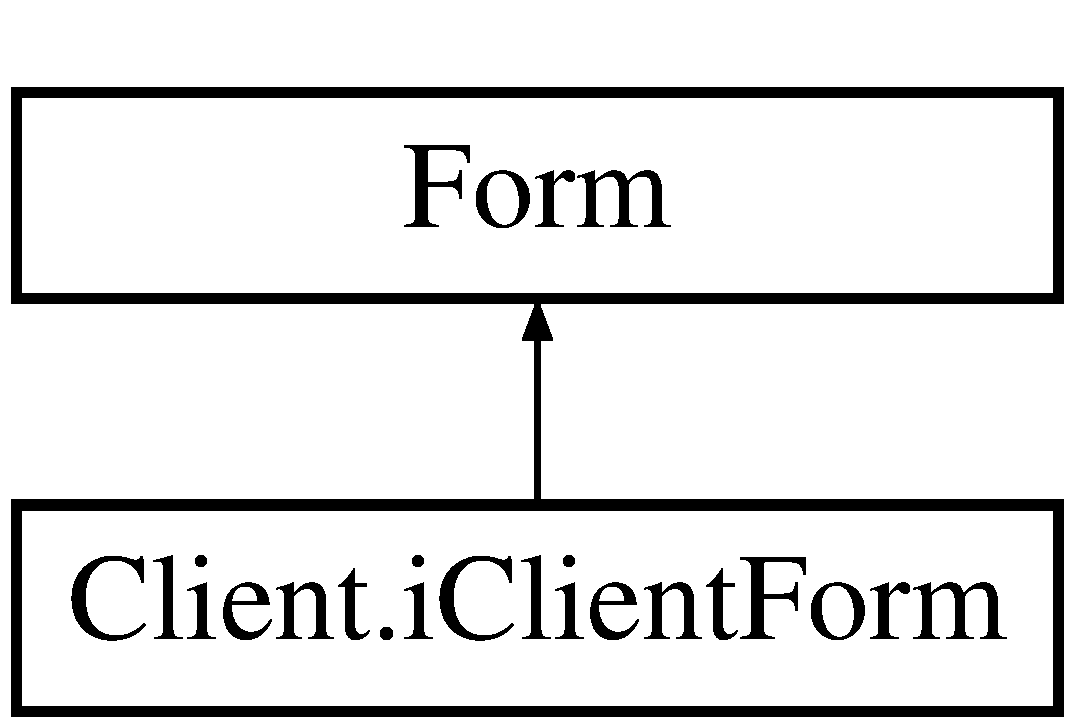
\includegraphics[height=2.000000cm]{class_client_1_1i_client_form}
\end{center}
\end{figure}
\subsection*{Public Member Functions}
\begin{DoxyCompactItemize}
\item 
\mbox{\hyperlink{class_client_1_1i_client_form_a02a4efefdc76771e7781b4b30e598465}{i\+Client\+Form}} ()
\begin{DoxyCompactList}\small\item\em Creates the actual client form \end{DoxyCompactList}\end{DoxyCompactItemize}
\subsection*{Protected Member Functions}
\begin{DoxyCompactItemize}
\item 
override void \mbox{\hyperlink{class_client_1_1i_client_form_a12dd32ccdf0e36d4e350fc51de41ce7b}{Dispose}} (bool disposing)
\begin{DoxyCompactList}\small\item\em Clean up any resources being used. \end{DoxyCompactList}\end{DoxyCompactItemize}


\subsection{Detailed Description}
\mbox{\hyperlink{namespacei_client}{i\+Client}} Form 



\subsection{Constructor \& Destructor Documentation}
\mbox{\Hypertarget{class_client_1_1i_client_form_a02a4efefdc76771e7781b4b30e598465}\label{class_client_1_1i_client_form_a02a4efefdc76771e7781b4b30e598465}} 
\index{Client\+::i\+Client\+Form@{Client\+::i\+Client\+Form}!i\+Client\+Form@{i\+Client\+Form}}
\index{i\+Client\+Form@{i\+Client\+Form}!Client\+::i\+Client\+Form@{Client\+::i\+Client\+Form}}
\subsubsection{\texorpdfstring{i\+Client\+Form()}{iClientForm()}}
{\footnotesize\ttfamily Client.\+i\+Client\+Form.\+i\+Client\+Form (\begin{DoxyParamCaption}{ }\end{DoxyParamCaption})}



Creates the actual client form 



\subsection{Member Function Documentation}
\mbox{\Hypertarget{class_client_1_1i_client_form_a12dd32ccdf0e36d4e350fc51de41ce7b}\label{class_client_1_1i_client_form_a12dd32ccdf0e36d4e350fc51de41ce7b}} 
\index{Client\+::i\+Client\+Form@{Client\+::i\+Client\+Form}!Dispose@{Dispose}}
\index{Dispose@{Dispose}!Client\+::i\+Client\+Form@{Client\+::i\+Client\+Form}}
\subsubsection{\texorpdfstring{Dispose()}{Dispose()}}
{\footnotesize\ttfamily override void Client.\+i\+Client\+Form.\+Dispose (\begin{DoxyParamCaption}\item[{bool}]{disposing }\end{DoxyParamCaption})\hspace{0.3cm}{\ttfamily [protected]}}



Clean up any resources being used. 


\begin{DoxyParams}{Parameters}
{\em disposing} & true if managed resources should be disposed; otherwise, false.\\
\hline
\end{DoxyParams}


The documentation for this class was generated from the following files\+:\begin{DoxyCompactItemize}
\item 
Client/\mbox{\hyperlink{i_client_form_8cs}{i\+Client\+Form.\+cs}}\item 
Client/\mbox{\hyperlink{i_client_form_8_designer_8cs}{i\+Client\+Form.\+Designer.\+cs}}\end{DoxyCompactItemize}

\chapter{File Documentation}
\hypertarget{i_client_form_8cs}{}\section{Client/i\+Client\+Form.cs File Reference}
\label{i_client_form_8cs}\index{Client/i\+Client\+Form.\+cs@{Client/i\+Client\+Form.\+cs}}
\subsection*{Classes}
\begin{DoxyCompactItemize}
\item 
class \mbox{\hyperlink{class_client_1_1i_client_form}{Client.\+i\+Client\+Form}}
\begin{DoxyCompactList}\small\item\em \mbox{\hyperlink{namespacei_client}{i\+Client}} Form \end{DoxyCompactList}\end{DoxyCompactItemize}
\subsection*{Namespaces}
\begin{DoxyCompactItemize}
\item 
namespace \mbox{\hyperlink{namespace_client}{Client}}
\begin{DoxyCompactList}\small\item\em \mbox{\hyperlink{namespace_client}{Client}} Name Space Holds the methods to run the iclient \end{DoxyCompactList}\end{DoxyCompactItemize}

\hypertarget{i_client_form_8_designer_8cs}{}\section{Client/i\+Client\+Form.Designer.\+cs File Reference}
\label{i_client_form_8_designer_8cs}\index{Client/i\+Client\+Form.\+Designer.\+cs@{Client/i\+Client\+Form.\+Designer.\+cs}}
\subsection*{Classes}
\begin{DoxyCompactItemize}
\item 
class \mbox{\hyperlink{class_client_1_1i_client_form}{Client.\+i\+Client\+Form}}
\begin{DoxyCompactList}\small\item\em \mbox{\hyperlink{namespacei_client}{i\+Client}} Form \end{DoxyCompactList}\end{DoxyCompactItemize}
\subsection*{Namespaces}
\begin{DoxyCompactItemize}
\item 
namespace \mbox{\hyperlink{namespace_client}{Client}}
\begin{DoxyCompactList}\small\item\em \mbox{\hyperlink{namespace_client}{Client}} Name Space Holds the methods to run the iclient \end{DoxyCompactList}\end{DoxyCompactItemize}

\hypertarget{_temporary_generated_file__036_c0_b5_b-1481-4323-8_d20-8_f5_a_d_c_b23_d92_8cs}{}\section{Client/obj/\+Debug/\+Temporary\+Generated\+File\+\_\+036\+C0\+B5\+B-\/1481-\/4323-\/8\+D20-\/8\+F5\+A\+D\+C\+B23\+D92.cs File Reference}
\label{_temporary_generated_file__036_c0_b5_b-1481-4323-8_d20-8_f5_a_d_c_b23_d92_8cs}\index{Client/obj/\+Debug/\+Temporary\+Generated\+File\+\_\+036\+C0\+B5\+B-\/1481-\/4323-\/8\+D20-\/8\+F5\+A\+D\+C\+B23\+D92.\+cs@{Client/obj/\+Debug/\+Temporary\+Generated\+File\+\_\+036\+C0\+B5\+B-\/1481-\/4323-\/8\+D20-\/8\+F5\+A\+D\+C\+B23\+D92.\+cs}}

\hypertarget{_temporary_generated_file__5937a670-0e60-4077-877b-f7221da3dda1_8cs}{}\section{Client/obj/\+Debug/\+Temporary\+Generated\+File\+\_\+5937a670-\/0e60-\/4077-\/877b-\/f7221da3dda1.cs File Reference}
\label{_temporary_generated_file__5937a670-0e60-4077-877b-f7221da3dda1_8cs}\index{Client/obj/\+Debug/\+Temporary\+Generated\+File\+\_\+5937a670-\/0e60-\/4077-\/877b-\/f7221da3dda1.\+cs@{Client/obj/\+Debug/\+Temporary\+Generated\+File\+\_\+5937a670-\/0e60-\/4077-\/877b-\/f7221da3dda1.\+cs}}

\hypertarget{_temporary_generated_file___e7_a71_f73-0_f8_d-4_b9_b-_b56_e-8_e70_b10_b_c5_d3_8cs}{}\section{Client/obj/\+Debug/\+Temporary\+Generated\+File\+\_\+\+E7\+A71\+F73-\/0\+F8\+D-\/4\+B9\+B-\/\+B56\+E-\/8\+E70\+B10\+B\+C5\+D3.cs File Reference}
\label{_temporary_generated_file___e7_a71_f73-0_f8_d-4_b9_b-_b56_e-8_e70_b10_b_c5_d3_8cs}\index{Client/obj/\+Debug/\+Temporary\+Generated\+File\+\_\+\+E7\+A71\+F73-\/0\+F8\+D-\/4\+B9\+B-\/\+B56\+E-\/8\+E70\+B10\+B\+C5\+D3.\+cs@{Client/obj/\+Debug/\+Temporary\+Generated\+File\+\_\+\+E7\+A71\+F73-\/0\+F8\+D-\/4\+B9\+B-\/\+B56\+E-\/8\+E70\+B10\+B\+C5\+D3.\+cs}}

\hypertarget{_program_8cs}{}\section{Client/\+Program.cs File Reference}
\label{_program_8cs}\index{Client/\+Program.\+cs@{Client/\+Program.\+cs}}
\subsection*{Classes}
\begin{DoxyCompactItemize}
\item 
class {\bfseries Client.\+Program}
\end{DoxyCompactItemize}
\subsection*{Namespaces}
\begin{DoxyCompactItemize}
\item 
namespace \mbox{\hyperlink{namespace_client}{Client}}
\end{DoxyCompactItemize}

\hypertarget{_assembly_info_8cs}{}\section{Client/\+Properties/\+Assembly\+Info.cs File Reference}
\label{_assembly_info_8cs}\index{Client/\+Properties/\+Assembly\+Info.\+cs@{Client/\+Properties/\+Assembly\+Info.\+cs}}

\hypertarget{_resources_8_designer_8cs}{}\section{Client/\+Properties/\+Resources.Designer.\+cs File Reference}
\label{_resources_8_designer_8cs}\index{Client/\+Properties/\+Resources.\+Designer.\+cs@{Client/\+Properties/\+Resources.\+Designer.\+cs}}
\subsection*{Classes}
\begin{DoxyCompactItemize}
\item 
class {\bfseries i\+Client.\+Properties.\+Resources}
\begin{DoxyCompactList}\small\item\em A strongly-\/typed resource class, for looking up localized strings, etc. \end{DoxyCompactList}\end{DoxyCompactItemize}
\subsection*{Namespaces}
\begin{DoxyCompactItemize}
\item 
namespace \mbox{\hyperlink{namespacei_client_1_1_properties}{i\+Client.\+Properties}}
\end{DoxyCompactItemize}

\hypertarget{_settings_8_designer_8cs}{}\section{Client/\+Properties/\+Settings.Designer.\+cs File Reference}
\label{_settings_8_designer_8cs}\index{Client/\+Properties/\+Settings.\+Designer.\+cs@{Client/\+Properties/\+Settings.\+Designer.\+cs}}
\subsection*{Classes}
\begin{DoxyCompactItemize}
\item 
class {\bfseries Client.\+Properties.\+Settings}
\end{DoxyCompactItemize}
\subsection*{Namespaces}
\begin{DoxyCompactItemize}
\item 
namespace \mbox{\hyperlink{namespace_client_1_1_properties}{Client.\+Properties}}
\end{DoxyCompactItemize}

%--- End generated contents ---

% Index
\backmatter
\newpage
\phantomsection
\clearemptydoublepage
\addcontentsline{toc}{chapter}{Index}
\printindex

\end{document}
